% presentation summary
\documentclass[a4paper, 10pt, twocolumn]{article}
\usepackage[top=2.5cm, bottom=2.5cm, left=2.5cm, right=2.5cm]{geometry}
\usepackage{times}
\usepackage{sectsty}
\pagenumbering{gobble}
\renewcommand\thesection{\Roman{section}}
\usepackage[dvipdfmx]{graphicx}
\usepackage{float}
\usepackage{setspace}
\usepackage{titlesec}
\usepackage{caption}
\usepackage{CJKutf8}
\usepackage[dvipdfmx, colorlinks=true, 
			linkcolor=blue, citecolor=red,
			bookmarks=true, bookmarkstype=toc]{hyperref}
\usepackage[font=scriptsize,labelfont=bf]{caption}
%\titlespacing\section{0pt}{12pt plus 4pt minus 2pt}{0pt plus 2pt minus 2pt}
\usepackage{amsmath}

\makeatletter
\def\@biblabel#1{(#1)}
\def\@cite#1{\textsuperscript{(#1)}}
\makeatother

\title{\begin{CJK}{UTF8}{min} $B%_%e!<%*%sEE;RE>49<B83$K$h$kJ|<M@~4D6-2<$K$*$1$kD6EAF3%=%l%N%$%I$K4X$9$k8&5f(B\end{CJK}}
\author{\begin{CJK}{UTF8}{min} ~~~~~~~~~~~~~~~~~~~~~~~~~~~~~~~~~~~~~~~~~~~~~~~~~~~~~~~~~~~~~~~~~~~~~~~~~~~~~~~~~~~~~~~~~~~~~~~~~~~~~~~~~~~~~~~~~~~~~~~~~~~~~                               ~~~$BML(B $B3p(B\end{CJK}}
\date{}

\sectionfont{\fontsize{9}{15}\selectfont}

\begin{document}

\maketitle

\section{Introduction}
~~~~Since the last particle of Standard Model, Higgs boson, it still remains us unsolved problems such as dark matter, neutrino oscillation, Higg's mass and etc.
However, these problems are able to be solved by including the physics beyond the Standard Model (BSM).
The BSM is possible to be observed through a rare process called charged lepton flavor violation (cLFV), which is still not found.

The branching ratio of cLFV is predicted to $\textless$ 10$^{-54}$ in terms of the neutrino oscillation, otherwise, the prediction of SUSY-GUT and SUSY-Seasaw is less than 10$^{-13}$ according to a mixing of slepton.
The cLFV seeking experiment has a history of 70 years.
Latest upper limit of experimental sensitivity is 5.7$\times$10$^{-13}$ (90\% C.L.), which is updated by MEG experiment for searching $\mu^+ \rightarrow e^+\gamma$, and nothing interesting is found in that region.

A coherent muon to electron transition (COMET) experiment is aiming to achieve the branching ratio of $\textless$ 3$\times$10$^{-17}$ to search the cLFV and BSM.
Different from the MEG experiment, COMET experiment intends to search for the direct $\mu \rightarrow e$ conversion with aluminium stopping target.
Thus, the experimental sensitivity totally depends on the muon beam quality.

To obtain that sensitivity, about 10$^{11}$ $\mu^-$/sec muons with low momentum are required at least for COMET experiment.
It can be achieved by using high intense proton beam and superconducting magnet system.
Considering the degradation of superconducting magnets under the high radiation environment, the radiation resistance and its thermal property is studied in this paper.

\section{Design}
~~~~COMET superconducting magnet system consists of pion capture solenoid, muon transport solenoid and detector solenoid for phase-I experiment.
The pion capture solenoid provides 5 Tesla to capture the pions produced from production target, muon transport solenoid and detector solenoid transport muons from pion decay to stopping target and track the signal of 105 MeV electron from $\mu^- \rightarrow e^-$ conversion with 3 Tesla and 1 Tesla.
These magnetic field must be smooth to eliminate the trapping of charged particle.

To reduce the costs and stored energy, the two coils of pion capture solenoid, CS0 and CS1, are designed close to the production target with radius of 672 mm, which works under high radiation and magnetic field.
As for the radiation issue, the conduction cooling is employed due to the reaction $^3$He(n,p)$^3$H, and the conductor is stabilized by pure Al to reduced the energy deposition and mass in pion capture solenoid.

\section{Simulation and Experiment}
~~~~The prompt radiation of phase-II and residual radiation of phase-I experiment are investigated by Monte Carlo code (GEANT4\cite{geant}, PHITS\cite{phits} and FLUKA\cite{fluka}) with different physics model and realistic geometry for phase-I experiment.
The magnetic field map for simulation is calculated by finite element method (FEM) with iron yoke.
As a result shown in figure~\ref{geo}, about 2.35$\times$10$^{21}$ n/m$^2$ neutrons ($\textgreater$ 1 MeV) at peak deposits in CS1 coil for 280-day operation.
In addition, over 2$\times$10$^7$ n/cm$^2$/sec neutrons with low energy will leak into detector room.
\begin{figure}[H]
 \centering
 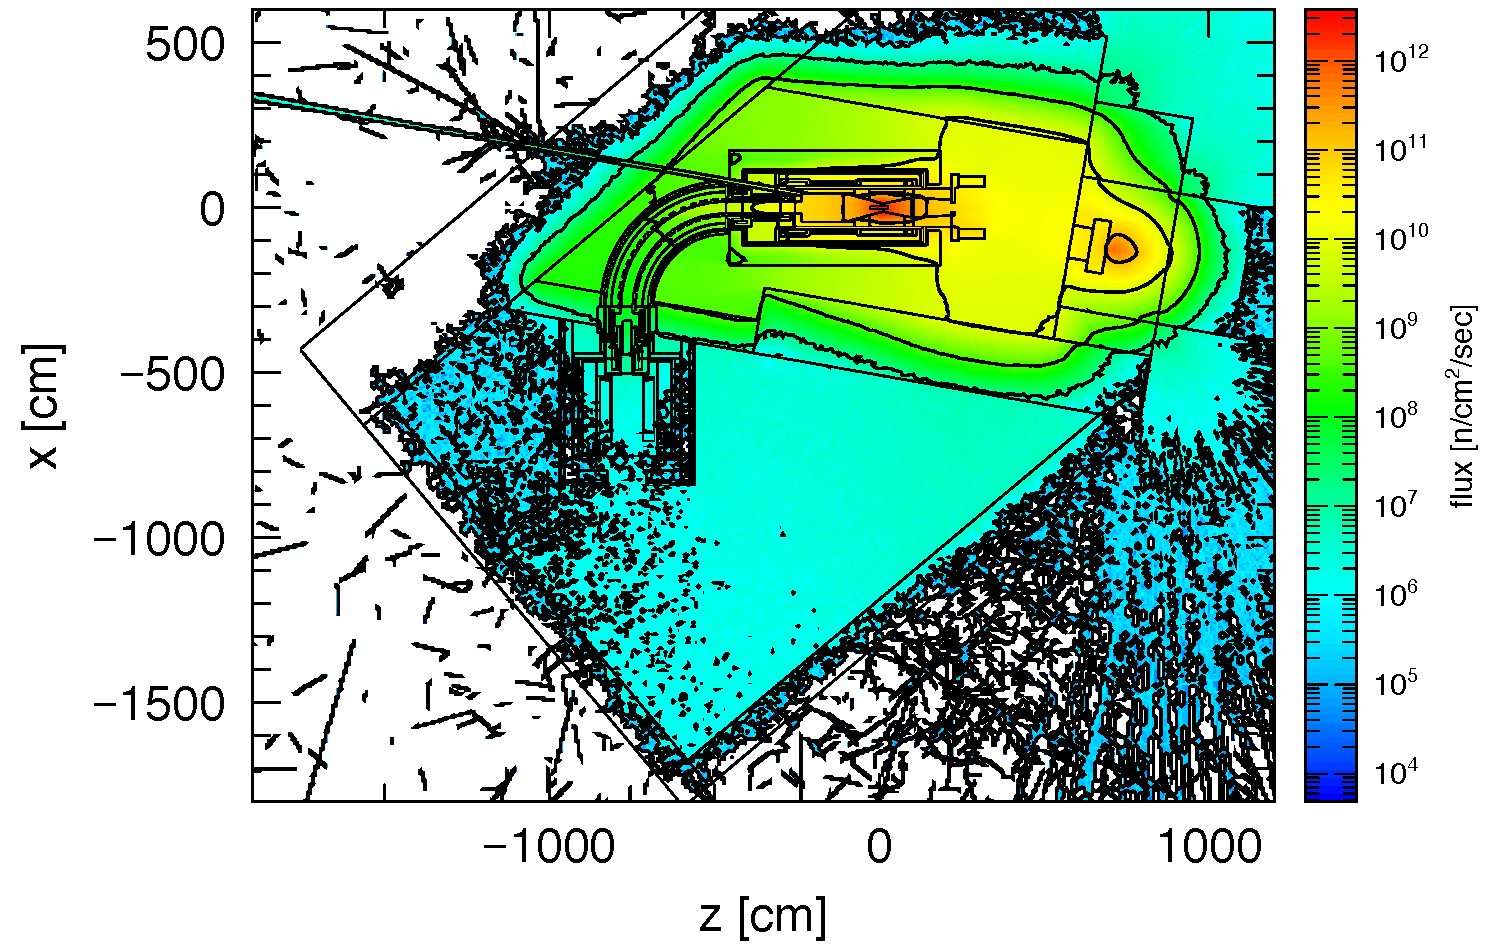
\includegraphics[scale=0.3]{fig/neutron.pdf}
 \caption{Neutron distribution of COMET phase-II experiment. It calculated by PHITS code with phase-I geometry but phase-II production target (pure tungsten) and proton intensity (4.4$\times$10$^{13}$ pps).}
 \label{geo}
\end{figure}
The residual radiation is estimated to 3.74 mSv/h at peak and 10 $\mu$Sv/h at 5 m far from the upstream of target after 30-day operation and 300-day cooling, which indicates it is difficult to take maintenance at the end of phase-I experiment.

Due to the cost issue, a radiation shield is optimized to replace the pure tungsten shield to protect the superconducting coils for both phase-I and phase-II experiment.
New radiation shield consists of stainless steel, copper and tungsten alloy with polygonal shape, which shown in figure~\ref{shield}.
The peak of DPA, neutron fluence and energy deposition in CS1 coil of this new shield is not changed, compared with all tungsten alloy shield.
Each peak of energy deposition, neutron fluence and DPA for 280-day operation are estimated to 0.8 MGy, 2.35$\times$10$^{21}$ n/m$^2$ and 1.11$\times$10$^{-5}$ DPA, respectively.
\begin{figure}[H]
 \centering
 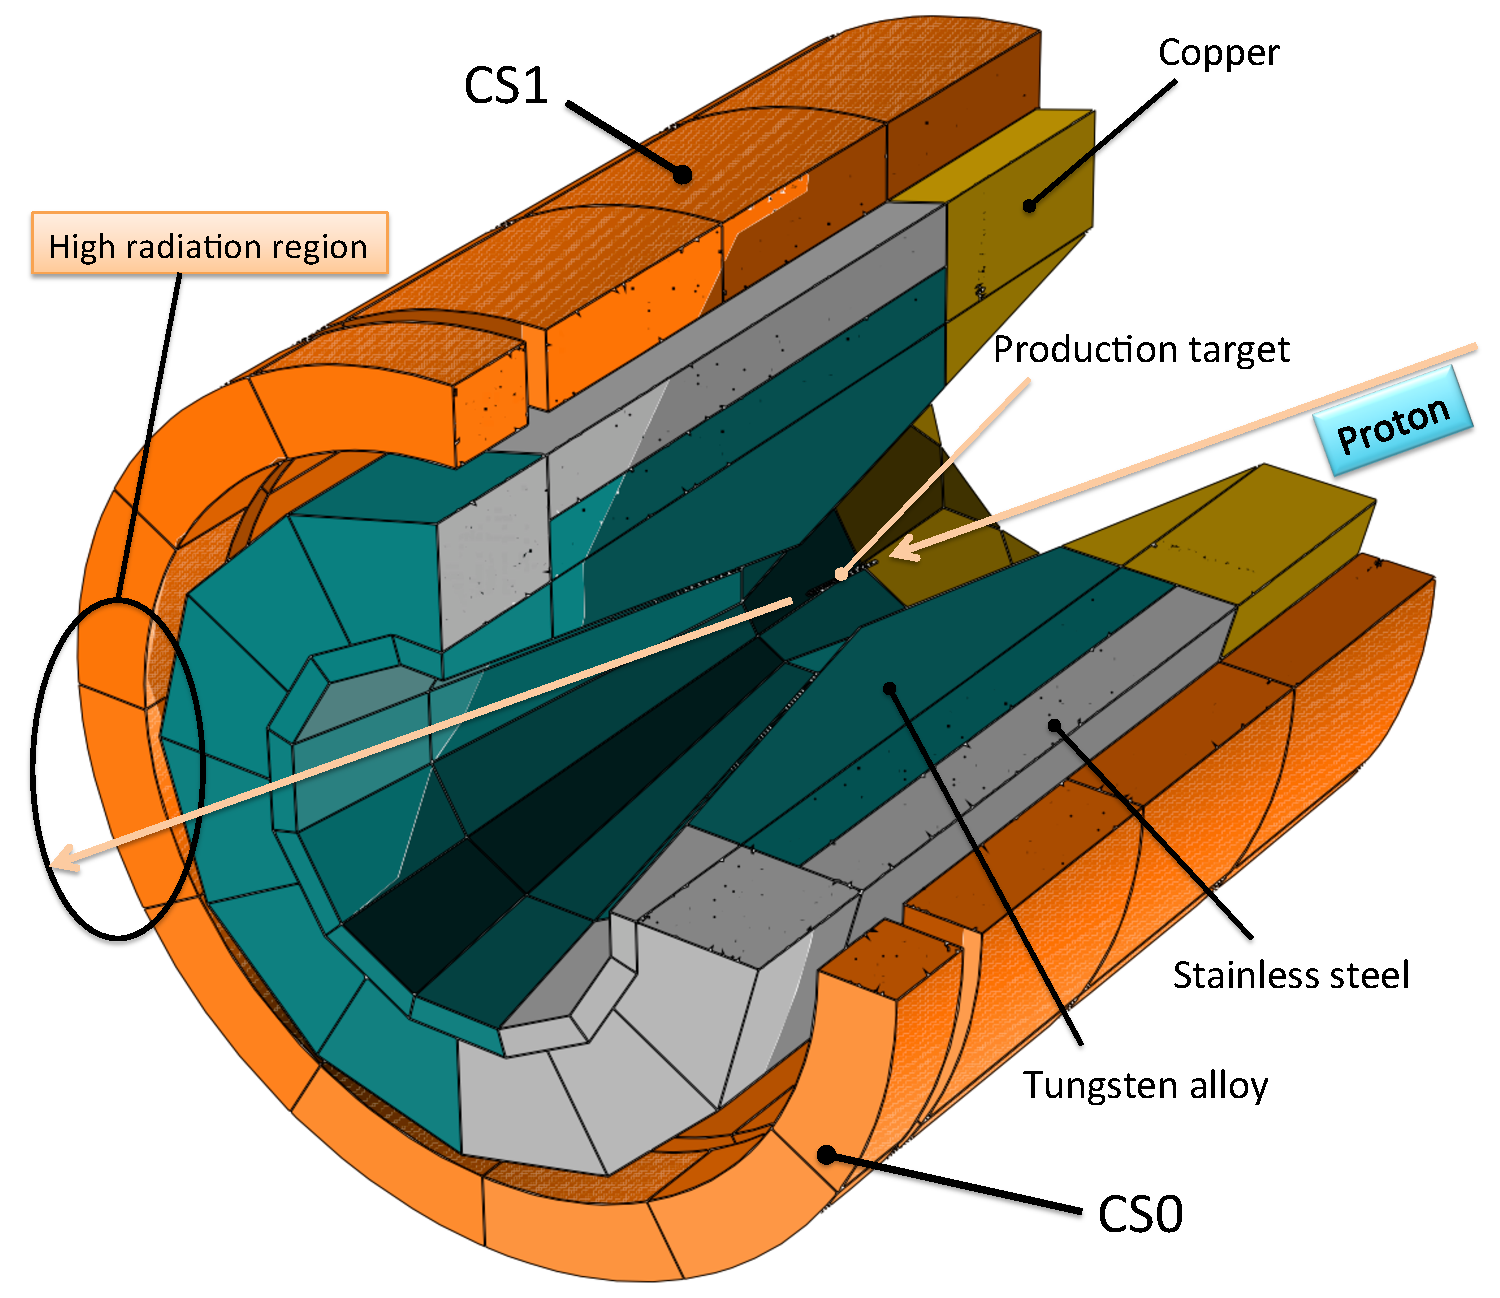
\includegraphics[scale=0.2]{fig/shielding.pdf}
 \caption{A new radiation shield consists of SUS304, copper and tungsten alloy for COMET experiment.}
 \label{shield}
\end{figure}

\subsubsection*{Experiment}
~~~~Since the superconducting magnet is exposed under high radiation, it may cause the degradation of superconducting coils, which has risk of quench.
To investigate the degradation of pure aluminium which used as stabilizer and cooling strips, the aluminium and copper is irradiated with 10$^{21}$ n/m$^2$ reactor neutrons totally.
As a result, the resistivity of aluminium and copper increase about 0.03 n$\Omega\cdot$m and 0.01 n$\Omega\cdot$m.

The insulation tape is covered the conductor as ground insulation.
It is developed by covering boron free glass on polyimide film with BT and epoxy resin to enhance the radiation resistance and mechanical property.
Its mechanical property is tested with and without irradiation.
The maximum tensile strength is about 9 MPa, and its tensile strength will not reduce after 10 MGy cobalt irradiation.

GFRPs are employed as the spacer in superconducting solenoid.
4 kinds of candidates, G10, CE, BMI and BT, are irradiated with electron with energy of 1 MeV and 34 MeV until 200 MGy and 4500 MGy, respectively.
BT has best radiation resistance and mechanical property among these samples, which shows its tensile strength is 350 MPa without irradiation, and almost keep it until 200 MGy irradiation.

%\begin{figure}[H]
% \centering
% 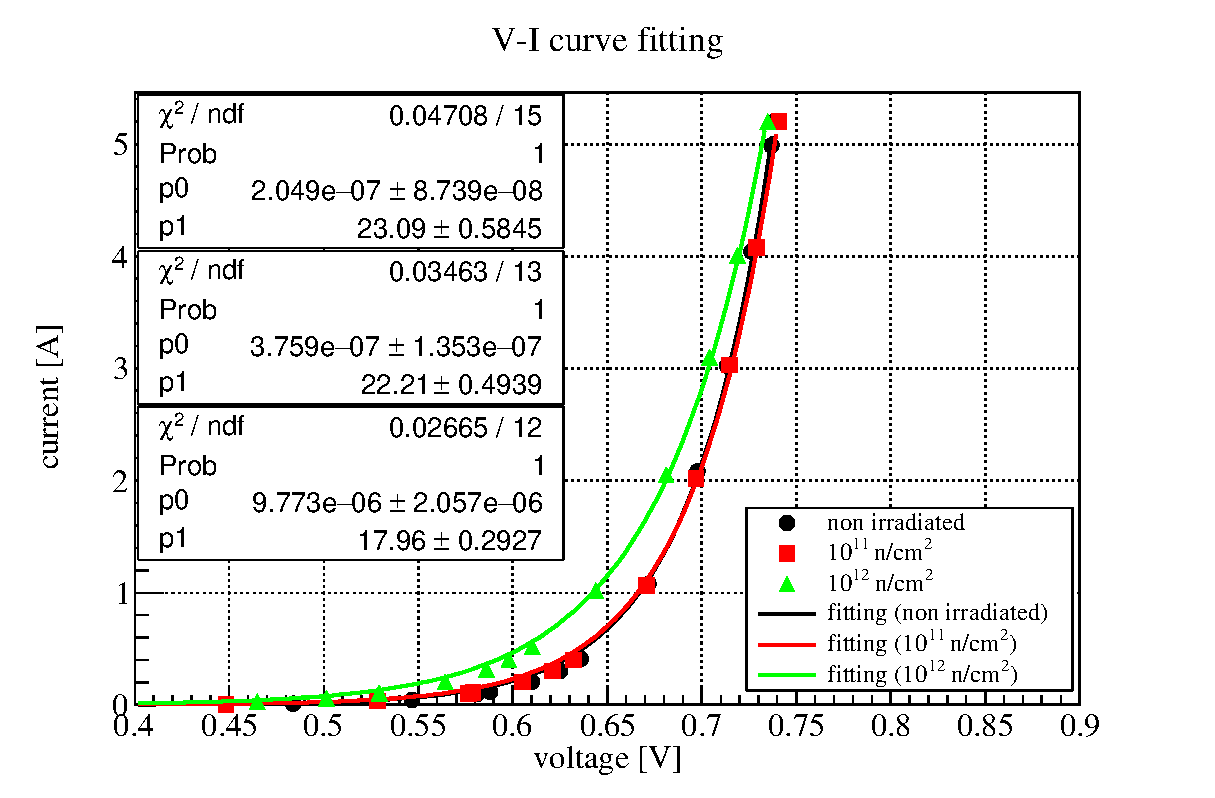
\includegraphics[scale=0.4]{fig/diodefit.eps}
% \caption{Measured and fitted the turn-on voltage before and after irradiation for quench protection diode.}
% \label{diode}
%\end{figure}
Quench protection diode is a switch of the quench protection circuit.
It irradiation test is taken by using secondary neutrons produced from reaction of (d,xn).
The neutron flux is measured by activation of Au, Al and Ni, which is estimated for 10$^{12}$ n/cm$^2$ totally until the end of experiment.
However, its turn-on voltage has no big change before and after irradiation.
%Figure~\ref{diode} shows its turn-on voltage has no big change before and after irradiation.
Its cryogenic property is also investigated on the liquid nitrogen temperature.
The turn-on voltage increases from 0.6 V to 1.1 V at 77 K.
In the real case, its voltage will increase up to 1.5 V at 210 A, 4.2 K under 10$^{12}$ n/cm$^2$ fast neutron irradiation by fitting the V-I curve.
The temperature will rise to about 11 K during the operation.

\subsubsection*{Thermal property}
~~~~Since the superconducting solenoid has a risk of quench when it exceeds to the current sharing temperature during the operation, its temperature is estimated based on the neutron irradiation test.
As for the original design, in figure~\ref{temp}, the temperature will rise to the current sharing temperature, 6.5 K, after 20-day operation.
To solve this issue, the design is optimized by inserting the Al strips from two sides, shortening the Al strip from edge to cooling pipe and enlarging the thickness of inner Al strip to 3 mm.
The 60-day operation becomes available after the optimization.
\begin{figure}[H]
 \centering
 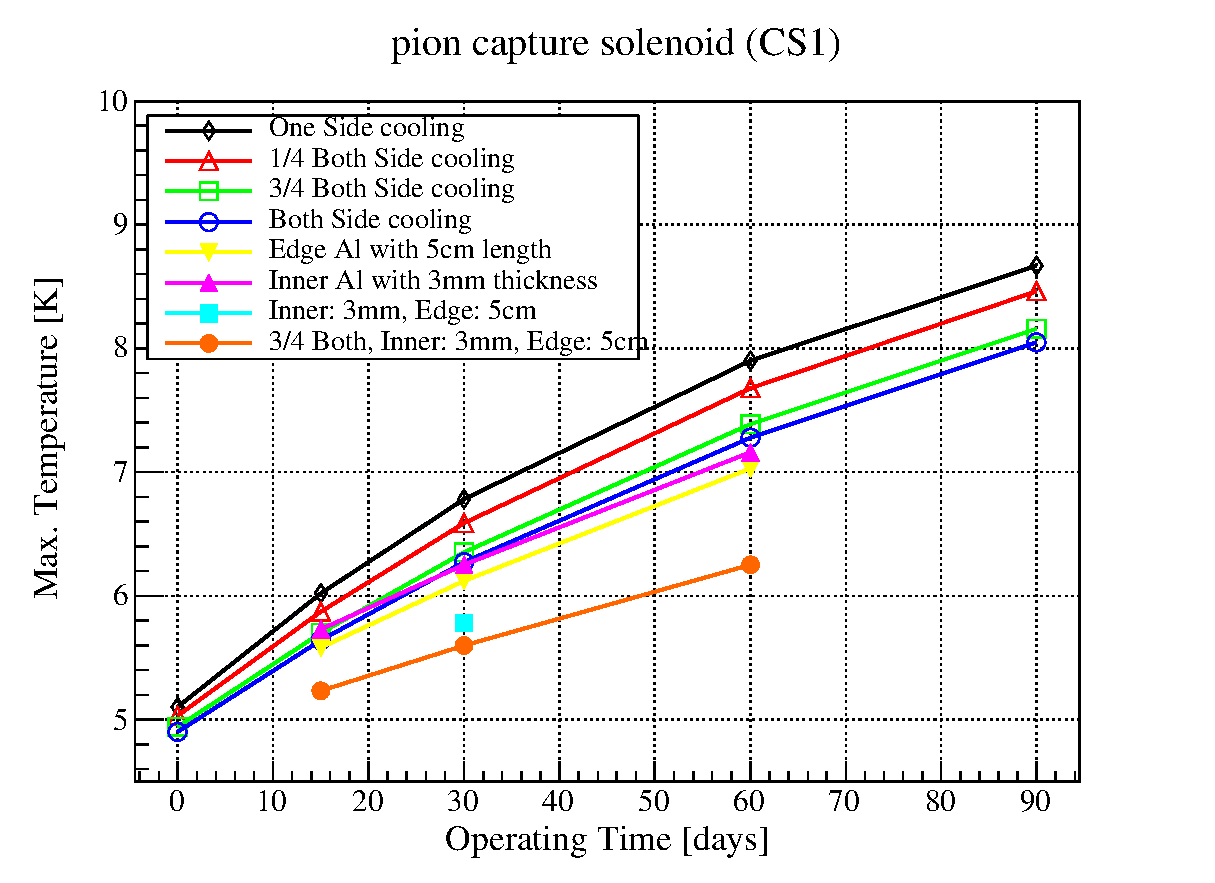
\includegraphics[scale=0.4]{fig/maxtemp.eps}
 \caption{The maximum temperature during the operation. Black line: original design, orange line: optimized design.}
 \label{temp}
\end{figure}

The maximum temperature after quench is estimated by MIITs calculation.
Electrical resistivity and specific heat of copper, aluminium and NbTi are fitted in terms of the experimental data.
As a result, the MIITs is estimated to 250 MA$^2\cdot$sec, which corresponds to 270 K after quench when the RRR of aluminium drops to 100.
To reduce the temperature after quench, the power supply should be increase to 600 V.

\section{Conclusion and Discussion}
~~~~In this study, the radiation and the radiation induced degradation of pion capture solenoid are estimated.
As for current design, the superconducting solenoid is able to work for 60 days continuously.
The maximum temperature after quench is not big issue, and it can be suppressed.
In COMET phase-II experiment, the superconducting solenoid is able to be operated until quench.

\begin{thebibliography}{10}
	\bibitem{phits} T. Sato, et al.: J. Nucl. Sci. Technol., 50:9 (2013), 913-923.
	\bibitem{fluka} T.T. B$\ddot{o}$hlen, et al.: Nucl. Data Sheets, 120 (2014), 211-214.
	\bibitem{geant} S. Agostinelli, et al.: Nucl. Instrum. Methods Phys. Res. A, 506 (2003), 250-303.
\end{thebibliography}

\end{document}

